\header[v]{
    \headtitle{Le bicêtre} \label{le-bicetre}
    %

    \insertComment{En 1633, Louis XIII bâtit, sur les ruines de l'ancien château Bicêtre, un hôpital pour les militaires invalides.}{Chanson écrite par Alphonse Besan\c con entre 1846 et 1851.}
    %, qui a été un hôpital, un asile d'aliénés et une prison parisienne
}

\enluminure{4}{\href{https://www.youtube.com/watch?v=TYN-ljmZSj8}{D}}{ans} ce Bicêtre, où l'on s'embête,
\\Loin de Paris que je regrette,
\\J'ai bien souvent, et longtemps médité
\\Sur la vieillesse et la caducité.
\\Amis, amis, apprenez à connaître
\\Ce vieux refrain, ce refrain de Bicêtre.
\\\\\textbf{Refrain :}
\\On n'peut pas bander toujours,
\\Il faut jouir de ses roupettes.
\\On n'peut pas bander toujours,
\\Il faut jouir de ses amours.
\\\\D'un vieux, un jour, j'tenais la quéquette,
\\La sonde en main, de l'autre la cuvette.
\\Pendant ce temps mon esprit méditait
\\Ce que tout bas le vieillard me disait :
\\"Prenez bien soin de vos pauvres gogottes,
\\Un jour viendra où vous pisserez sur vos bottes."
\\\\Idiots, fous, épileptiques
\\Sont des arguments sans réplique :
\\Tout dépérit le pauvre genre humain
\\N'a plus d'espoir que dans le carabin.
\\Or, pour créer une race nouvelle,
\\Jamais, enfants, ne mouchez la chandelle.
\\\\A l'oeuvre, donc, jeunes athlètes,
\\Gaillardement, engrossez les fillettes.
\\Baisez, foutez, ne craignez nul écueil:
\\Quand on est jeune, il faut baiser à l'oeil.
\\Avec le temps, Vénus devient avare :
\\Aux pauvres vieux, le coup est cher et rare.
\breakpage
Quand la vieillesse, triste et caduque,
\\Vous foutra son pied à la nuque,
\\Quand votre vît, à jamais désossé,
\\Sur vos roustons pendra flasque et glacé:
\\Allez crier à la face du prêtre
\\Ce vieux refrain, ce refrain de Bicêtre.
\\
\bigskip
\begin{figure}[h!]
\centering
   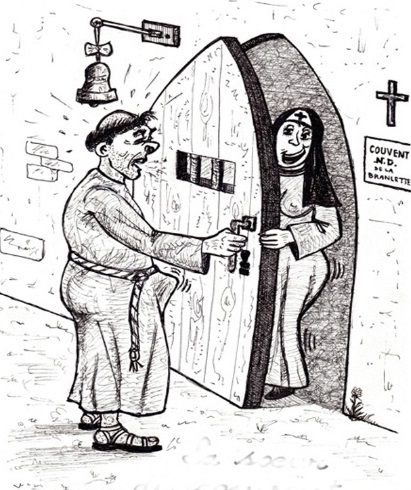
\includegraphics[width=0.9\textwidth]{images/bicetre.jpg}
 \end{figure}

\breakpage